\documentclass{ximera}

\newcommand{\RR}{\mathbb R}
\renewcommand{\d}{\,d}
\newcommand{\dd}[2][]{\frac{d #1}{d #2}}
\renewcommand{\l}{\ell}
\newcommand{\ddx}{\frac{d}{dx}}
\newcommand{\dfn}{\textbf}
\newcommand{\eval}[1]{\bigg[ #1 \bigg]}


\author{Jason Miller and Jim Talamo}
\license{Creative Commons 3.0 By-bC}


\outcome{}

\begin{document}
\begin{exercise}
%
%Two problems that require set up only, but each problem has a region where the inner and outer curve change and a region where there is an inner and outer curve (ex, r=2cos(2theta) and r=1, region 1 is region common to both curves, and region 2 is the region outside of r=1 but inside of r = 2 cos(2theta))

Consider the polar curves $r=2\sin(3\theta)$ (shown in blue) and $r=1$ (shown in red). 




\begin{image}  
  \begin{tikzpicture}  
    \begin{axis}[  
        xmin=-2.5,  
        xmax=3,  
        ymin=-2.5,  
        ymax=2.5,  
        axis lines=center,  
        xlabel=$x$,  
        ylabel=$y$,  
        every axis y label/.style={at=(current axis.above origin),anchor=south},  
        every axis x label/.style={at=(current axis.right of origin),anchor=west},axis on top
      ]  
      \addplot [data cs=polar, very thick, mark=none,fill=fill1,domain=10:50,samples=180,smooth] (x, {2*sin(3*x)});
      \addplot[data cs=polar, very thick, mark=none, fill=white,  domain=0:90, samples=180, smooth] (x, {1});
      \addplot[data cs=polar,penColor2,domain=0:360,samples=360,smooth, thick] (x,{2*sin(3*x)}) ;
      \addplot[data cs=polar, penColor, domain=0:360, samples=360, smooth, thick] (x, {1});      
            \end{axis}  
  \end{tikzpicture}  
\end{image} 

We want to set up an integral that expresses the area of the shaded region $S$ that lies inside the curve $r=2\sin(3\theta)$ but outside of the circle $r=1$ in the 1st quadrant. 





The area of the region $S$ is 

\[
\int_{\answer{\pi/18}}^{\answer{ 5\pi/18 } } \answer{ \frac{1}{2}\left[(2\sin(3\theta))^2-1\right]   } \d \theta=\answer{ \frac{\pi}{9}+\frac{\sqrt{3}}{6}}
\]





\begin{hint}

Consider a general polar curve $r=f(\theta)$ as below. 


\begin{image}
  \begin{tikzpicture}
\begin{axis}[
axis y line=middle,axis x line=middle,name=myplot,%
			%x=.37\marginparwidth,
			%y=.37\marginparwidth,
			%xtick={-1,1},
			%minor x tick num=1,% 
%			extra x ticks={.33},
%			extra x tick labels={$1/3$},
			%ytick={-1,1},
			%minor y tick num=1,%extra y ticks={-5,-3,...,7},%
			ymin=-.1,ymax=1.1,
			xmin=-.1,xmax=1.1, 
axis on top
]

\addplot [fill1,fill=fill1,area style, smooth,domain=18:72,samples=30] ({cos(x)*(1+.05*cos(9*x))},{sin(x)*(1+.05*cos(9*x))}) -- (axis cs:0,0) -- cycle;

\addplot [penColor2 ,thick, smooth,domain=0:90,samples=30] ({cos(x)*(1+.05*cos(9*x))},{sin(x)*(1+.05*cos(9*x))});


\addplot [fill1,fill=white ,area style, smooth,domain=12:64,samples=30] ({cos(x)*(.4+.05*cos(9*x))},{sin(x)*(.6+.05*cos(9*x))}) -- (axis cs:0,0) -- cycle;

\addplot [penColor,thick, smooth,domain=0:90,samples=30] ({cos(x)*(.4+.05*cos(9*x))},{sin(x)*(.6+.05*cos(9*x))});


\draw [thick,penColor,] (axis cs:0,0) -- (axis cs: 0.905831, 0.294322) node [pos=.8,below,rotate=18,black] { $\theta=\alpha$};

\draw [thick,penColor,] (axis cs:0,0) -- (axis cs:0.313792, 0.965751) node [pos=.8,above,rotate=72,black] { $\theta=\beta$};

\draw[very thick, orange] (axis cs:0,0) -- (axis cs:0.83, .65) node [pos=.8, above, rotate=40, orange] {$\theta=\theta_{0}$};


\draw (axis cs:.25, .37   ) node[penColor] {$ g(\theta)$};

\draw (axis cs:.8,.82) node[penColor2] { $f(\theta)$};


\end{axis}

\node [right] at (myplot.right of origin) { $\theta=0$};
\node [above] at (myplot.above origin) { $\theta=\pi/2$};
\end{tikzpicture}
\end{image}


The area enclosed by the polar curves $r=f(\theta)$ (in blue) and $r=g(\theta)$ (in red) from $\theta=\alpha$ to $\theta=\beta$ is given 

\[
\int_{\alpha}^{\beta} \frac{1}{2} (f(\theta)^2 -g(\theta)^2) \d \theta
\]

Consider a fixed angle $\theta=\theta_{0}$ (in orange). This ray extends from the origin outward and will intersect the two polar curves. Call the outermost curve that the ray intersects
$r_{outer}$ and call the innermost curve that the ray intersects $r_{inner}$. 

Then we express the area between two polar curves between $\alpha$ and $\beta$ as 

\[
\int_{\alpha}^{\beta} \frac{1}{2}( (r_{outer})^2 -(r_{inner})^2) \d \theta
\]


In our case (see below), we have $r_{outer}=1+\cos(\theta)$ and $r_{inner}=1$.




\begin{image}  
  \begin{tikzpicture}  
    \begin{axis}[  
        xmin=-2.5,  
        xmax=3,  
        ymin=-2.5,  
        ymax=2.5,  
        axis lines=center,  
        xlabel=$x$,  
        ylabel=$y$,  
        every axis y label/.style={at=(current axis.above origin),anchor=south},  
        every axis x label/.style={at=(current axis.right of origin),anchor=west},axis on top
      ]  
      \addplot [data cs=polar, very thick, mark=none,fill=fill1,domain=10:50,samples=180,smooth] (x, {2*sin(3*x)});
      \addplot[data cs=polar, very thick, mark=none, fill=white,  domain=0:90, samples=180, smooth] (x, {1});
      \addplot[data cs=polar,penColor2,domain=0:360,samples=360,smooth, thick] (x,{2*sin(3*x)}) ;
      \addplot[data cs=polar, penColor, domain=0:360, samples=360, smooth, thick] (x, {1});      
     \draw[very thick, orange] (axis cs:0,0) -- (axis cs:2, 1.55) node [pos=.9, above, rotate=40, orange] {$\theta=\theta_{0}$};
        \draw (axis cs:1.24, -1.47  ) node[penColor2] {$ r=2\cos(3\theta)$};
      \draw (axis cs:-1, -.89 ) node[penColor] {$r=1$};
            \end{axis}  
  \end{tikzpicture}  
\end{image} 


Now we need to identify the initial angle $\alpha$ and the final angle $\beta$ that bounds our region $S$. In order to determine these angles we need to think about how the curve is traced out as $\theta$ varies. 

Understanding how $r=1$ is traced out is the simplest. It is traced out in the standard fashion as $\theta$ varies. That is, for each value of $\theta$, the associated point on the curve is $(1, \theta)$ in polar coordinates. 

Let's graph $r=2\sin(3\theta)$ on $r$ and $\theta$ axes. 

\begin{image}  
  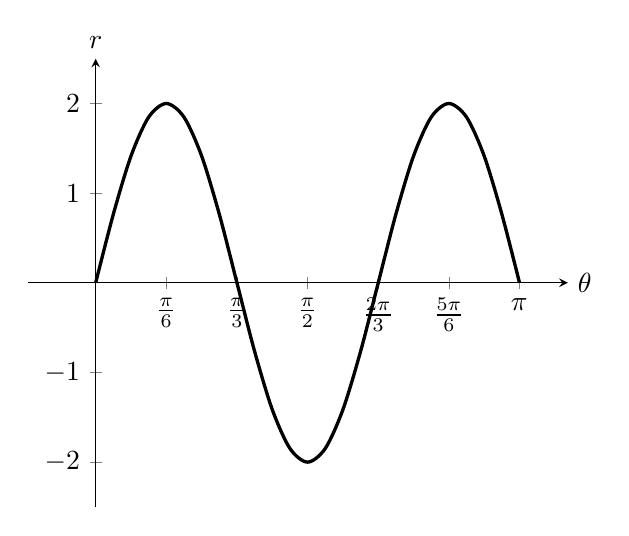
\begin{tikzpicture}  
    \begin{axis}[  
        xmin=-.5,  
        xmax=3.5,  
        ymin=-2.5,  
        ymax=2.5,  
        axis lines=center,  
        xlabel=$\theta$,  
        ylabel=$r$,  
        every axis y label/.style={at=(current axis.above origin),anchor=south},  
        every axis x label/.style={at=(current axis.right of origin),anchor=west},  
       xtick={ .523, 1.047, 1.57, 2.094, 2.618,  3.14   },
       xticklabels={ $\frac{\pi}{6}$, $\frac{\pi}{3}$, $\frac{\pi}{2}$, $\frac{2\pi}{3}$, $\frac{5\pi}{6}$, $\pi$ },
            ]  
      \addplot [ very thick, mark=none,domain=0:pi,smooth] {2*sin(deg(3*x))};
            \end{axis}  
  \end{tikzpicture}  
\end{image} 

Both curves can be traced out exactly once by letting $\theta$ vary from $0$ to $\pi$ (convince yourself of this!).

As $\theta$ goes from $0$ to $\frac{\pi}{3}$ we see that $r$ increase from $0$ to $2$ and then decreases from $2$ back down to $0$. This corresponds to the petal in the 1st quadrant. 

But we don't want the entire petal. So we need to find for which $\theta$ values the $r$ values of the two curves coincide. 

We set $r=2\sin(3\theta)$ and $r=1$ equal. 

Set $2\sin(3\theta)=1$.  Note that $\sin(\cdot) = 0$ when $(\cdot) = \frac{\pi}{2},\frac{5\pi}{2}, \ldots$  (meaning that we have to set the expression \emph{inside} the sine function equal to those values.  Doing this gives us that $3 \theta = \frac{\pi}{2},\frac{5\pi}{2}, \ldots$, so $\theta=\answer{\frac{\pi}{18}}$ and $\theta=\answer{\frac{5\pi}{18}}$ (list the $\theta$ values from smaller to larger. 


In order to evaluate the integral, recall the trig identity $\sin^2(\theta)=\frac{1-\cos(2\theta)}{2}$. 










\end{hint}

\end{exercise}
\end{document}
